\chapter{Hypothesis Generation}
\ifpdf
    \graphicspath{{Chapter2/Chapter2Figs/PNG/}{Chapter2/Chapter2Figs/PDF/}{Chapter2/Chapter2Figs/}}
\else
    \graphicspath{{Chapter2/Chapter2Figs/EPS/}{Chapter2/Chapter2Figs/}}
\fi

\section{Hypothesis Generation}

Hypothesis Generation phase is based on the following conjecture which we try to prove in the next subsection.

\begin{theorem}
 A point, $P$ inside a simple polygon sees atleast one edge of the polygon completely.
\end{theorem}
The proof of the above theorem comes from the following two simple facts.
\begin{itemize}
 \item An edge is partially visible from a point inside the polygon only if it is occluded partially by another reflex vertex of the polygon
not belonging to that edge.
\item A reflex vertex can occlude one and only one edge of the polygon.
\end{itemize}

To prove the theorem for any arbitrary polygon we obtain the visibility polygon of point P and show that atleast one edge of this
visibility polygon, which is also an edge of the original polygon, is completely visible from point $P$. Alternatively Theorem 1 can be
 restated as follows.

\begin{definition}
 {\bf Spurious Edge:} In the visibility polygon of a point, an edge is called a spurious edge if it is obtained by extending the line
 joining the point $P$ and a reflex vertex till it meets the polygon.
\end{definition}
Additional details about spurious edges and vertices can be obtained from \cite{key4}


\begin{theorem}
 The visibility polygon of a point $P$ has atleast one edge which completely overlaps with an edge of the original polygon.
\end{theorem}
{\bf Proof} Let the visibility polygon be $V$. Let the visibility polygon have $n$ non-spurious edges and $r$ spurious edges.
Each of the spurious edge is due to a reflex vertex, so the polygon would have $r$ reflex vertices at least.
 According to the theorem, one of the $n$ edges must overlap completely with an edge of the polygon.
We prove it by contradiction. Assume to the contrary that all of the $n$ edges are partially visible from $P$. Thus each of the $n$
edges must be occluded by a reflex vertex $v$ not lying on the edge. And since a reflex vertex cannot occlude multiple edges, therefore
 a total of $n$ reflex vertices will be required to occlude the $n$ edges.
So such a polygon, if it exists, should have $n+r$ reflex vertices, but it is not possible to construct a closed polygon with all
 vertices as reflex vertex.
Hence our original assumption was wrong.

\section{Algorithm}

\begin{enumerate}
 \item Iterate over the edges of the polygon and the edges of the map. and find an edge in the map which has the same length and
 orientation as an edge in the polygon.

 \item
 Translate the visibility polygon such that the matching edge of the map polygon
and the visibility polygon coincide.

 \item
 For each of the remaining edges of the visibility polygon, check whether a 
complete match exists or not. If all the remaining edges match, the point where the
origin was translated is added to the set of hypotheses.

\end{enumerate}

\newpage

\section{Examples}

\begin{figure}[h]
\begin{center}
\scalebox{0.40}{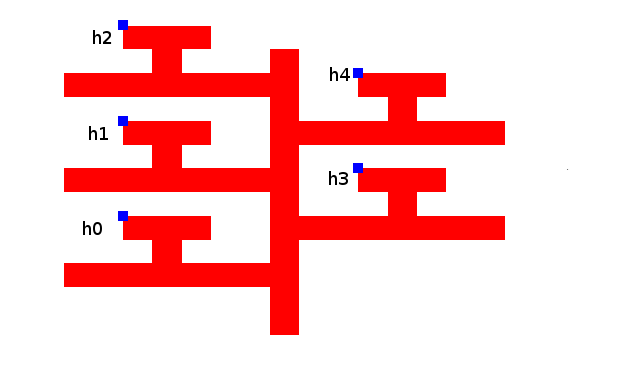
\includegraphics{Images/Hypothesis_office.png}}
\caption{\label{fig:Hypothesis Generation}Hypothesis Generation}
\end{center}
\end{figure}


\begin{figure}[h]
\begin{center}
\scalebox{0.40}{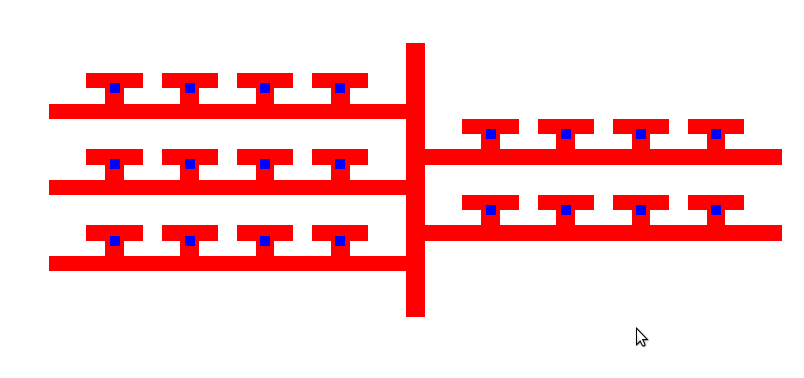
\includegraphics{Images/HypothesisOfficeAnti.png}}
\caption{\label{fig:Hypothesis Generation}Hypothesis Generation}
\end{center}
\end{figure}


% ------------------------------------------------------------------------

%%% Local Variables: 
%%% mode: latex
%%% TeX-master: "../thesis"
%%% End: 
